\documentclass{article}

%%%%
% PLOTS mapas y conglomerados
% bibliografia
%%%%
\usepackage[T1]{fontenc} %%%
\usepackage[utf8]{inputenc}
\usepackage{longtable}
\usepackage{authblk}
\usepackage{adjustbox}



\usepackage{natbib}

\title{LOS INDICES DE COLOMBIA}
% autores
\renewcommand\Authand{, y }
\author[1]{\normalsize MACQUEEN}


\affil[1,2]{\small  Escuela de Ingenier\'ia,Universidad de los Andes\\
\texttt{{delcurso,deallado}@uniandes.edu.col}}
\affil[1]{\small Instituto de altas investigaciones financieras\\
Banco del Parque\\
\texttt{delcurso@bp.com.col}}

\date{30 de Junio de 2018}

%%%%
\usepackage{Sweave}
\begin{document}
\Sconcordance{concordance:FinaldeR.tex:FinaldeR.Rnw:%
1 31 1 1 0 24 1 1 9 2 1 1 7 11 1 1 14 1 3 12 1 1 5 1 2 4 1 1 9 1 0 1 7 %
6 1 1 4 1 2 11 1 1 5 1 2 15 0 1 1 16 0 1 3 10 1 1 14 1 1 1 2 4 0 2 3 6 %
1 1 7 5 0 1 4 2 0 1 2 5 0 1 10 1 0 1 3 24 1}


\maketitle


\begin{abstract}
El proposito principal de este trabajo es describir los procesos para partir una poblacion N-dimensional en partes de k tama<U+00F1>o en forma de una muestra. El proceso, que se denomina 'k-means' aparece para dar particiones que son rasonablemente eficientes en el sentido de las variables dentro de las categorias. Eso es, que si p es la probabilidad de densidad para la poblaci<U+00F3>n S, S=s1,s2,...,Sn. La parte de En y de ui siendo i=1,2,3,..,k es el promedio condicional de p sobre S. Diremos de ahora en adelante en el documento 'tiende a ser bajo' para referirnos en principio a las consideraciones intuitivas y corroboradas del an<U+00E1>lisis matematico y practicas computacionales.
\end{abstract}

\section*{Introducci\'on}

The main purpose of this paper is to descrube a procces for partitioning an N-dimensional population into k sets on the basis of a sample. Th procvess, which is called 'k-means', appears to five partitions which are reasonably effcient in the sense of within-class variance. That is, if p is the probability mass functon for the population, S= S1,S2,..,Sn is a partition of En. We say 'tends to be low' primarily because of intutive considerations, corroborated to some extent by mthematical analysis and practical computational experience.


Comencemos viendo que hay en la secci\'on \ref{univariada} en la p\'agina \pageref{univariada}.

\clearpage



\section{Exploraci??n Univariada}\label{univariada}

En esta secci\'on exploro cada \'indice. En esta secci\'on exploro cada \'indice. En esta secci\'on exploro cada \'indice. En esta secci??n exploro cada ??ndice. En esta secci\'on exploro cada \'indice. En esta secci\'on exploro cada \'indice. En esta secci\'on exploro cada \'indice. En esta secci\'`n exploro cada \'indice. En esta secci\'on exploro cada \'indice.


Para conocer el comportamiento de las variables se ha preparado la Tabla \ref{Tfrecuencias}, donde se describe la distribuci\'on de las modalidades de cada variable. Los n\'umeros representan la situaci\'on de algun pa\'is en ese indicador, donde el mayor valor num\'erico es la mejor situaci\'on.


Como apreciamos en la Tabla \ref{Tfrecuencias}, los pa\'ises en la mejor situaci\'on son los menos, salvo en el caso del \emph{\'indice de libertas mundial}\footnote{N\'otese que esto se puede deber a la {\bf menor} cantidad de categor\'ias.}

\clearpage

Para resaltar lo anterior, tenemos la Figura \ref{barplots} en la p\'agina \pageref{barplots}. 


%%%%% figure
\begin{figure}[h]
\centering

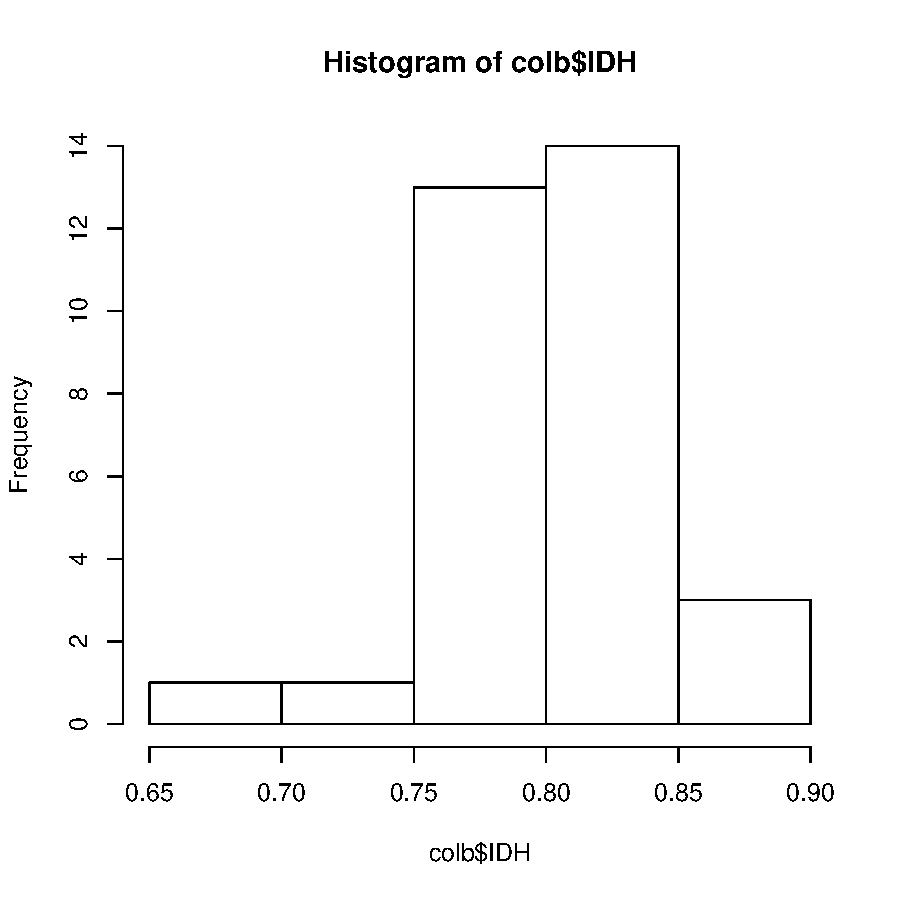
\includegraphics{FinaldeR-barplots}

\caption{Distribuci\'on de Indicadores}
\label{barplots}
\end{figure}

Adem\'as de la distribuci\'on de los variable, es importante saber el valor central. Como los valores son de naturaleza ordinal debemos pedir la {\bf mediana} y otras medidas de posici\'on (como los \emph{cuartiles}, los que no pediremos pues son pocos valores). La mediana de cada variable la mostramos en la Tabla \ref{stats} en la p\'agina \pageref{stats}.



\section{Exploraci\'on Bivariada}

En este trabajo estamos interesados en el impacto de los otros indices en el nivel de Democracia. Veamos las relaciones bivariadas que tiene esta variable con todas las dem\'as:

       cabeLog  restoLog
[1,] 0.4873974 0.1773112

Veamos la correlaci\'on entre las variables independientes:


         cabeLog restoLog
cabeLog  "1"     ""      
restoLog "0.84"  "1"     
Lo visto en la Tabla \ref{corrTableX} se refuerza claramente en la Figura \ref{corrPlotX}.

\begin{figure}[h]
\centering
\begin{adjustbox}{width=7cm,height=7cm,clip,trim=1.5cm 0.5cm 0cm 1.5cm}

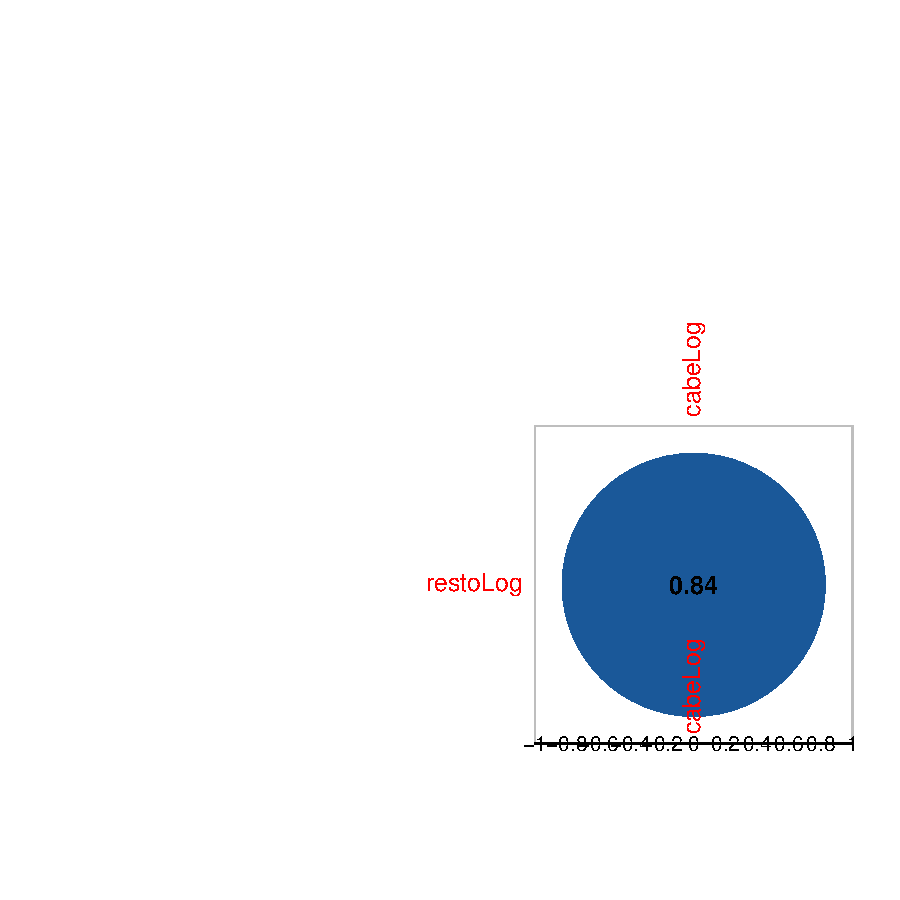
\includegraphics{FinaldeR-corrPlotX}
\end{adjustbox}
\caption{correlaci\'on entre predictores}
\label{corrPlotX}
\end{figure}


\clearpage

\section{Modelos de Regresi\'on}

Finalmente, vemos los modelos propuestos. Primero sin la libertad mundial como independiente, y luego con est\'a. Los resultados se muestran en la Tabla \ref{regresiones} de la p\'agina \pageref{regresiones}.


Call:
lm(formula = IDH ~ ., data = colb[, c(1, 7)])

Residuals:
      Min        1Q    Median        3Q       Max 
-0.113668 -0.018473  0.001249  0.016927  0.071401 

Coefficients:
            Estimate Std. Error t value Pr(>|t|)    
(Intercept) 0.634408   0.055163  11.501  1.6e-12 ***
cabeLog     0.012846   0.004202   3.057  0.00466 ** 
---
Signif. codes:  0 '***' 0.001 '**' 0.01 '*' 0.05 '.' 0.1 ' ' 1

Residual standard error: 0.03737 on 30 degrees of freedom
Multiple R-squared:  0.2376,	Adjusted R-squared:  0.2121 
F-statistic: 9.347 on 1 and 30 DF,  p-value: 0.004664Call:
lm(formula = IDH ~ ., data = colb[, c(1, 7:8)])

Residuals:
     Min       1Q   Median       3Q      Max 
-0.09489 -0.02041  0.00433  0.01740  0.06372 

Coefficients:
             Estimate Std. Error t value Pr(>|t|)    
(Intercept)  0.765665   0.064813  11.813 1.32e-12 ***
cabeLog      0.030664   0.006886   4.453 0.000116 ***
restoLog    -0.029571   0.009626  -3.072 0.004592 ** 
---
Signif. codes:  0 '***' 0.001 '**' 0.01 '*' 0.05 '.' 0.1 ' ' 1

Residual standard error: 0.03302 on 29 degrees of freedom
Multiple R-squared:  0.4247,	Adjusted R-squared:  0.3851 
F-statistic: 10.71 on 2 and 29 DF,  p-value: 0.0003296
Como se vi\'o en la Tabla \ref{regresiones}, cuando est\'a presente el \emph{indice de libertad mundial}, el \emph{\'indice de libertad de prensa} pierde significancia.

\clearpage

\section{Exploraci??n Espacial}

Como acabamos de ver en la Tabla \ref{regresiones} en la p\'agina \pageref{regresiones}, si quisieras sintetizar la multidimensionalidad de nuestros indicadores, podr\'iamos usar tres de las cuatro variables que tenemos (un par de las originales tiene demasiada correlaci\'on). 

As\'i, propongo que calculemos conglomerados de pa\'ises usando toda la informaci\'on de tres de los indicadores. Como nuestras variables son ordinales utilizaremos un proceso de conglomeraci??n donde las distancia ser\'an calculadas usando la medida {\bf gower} propuestas en \cite{gower_general_1971}, y para los enlazamientos usaremos la t??cnica de {\bf medoides} seg\'un \cite{reynolds_clustering_2006}. Los tres conglomerados se muestran en la Figura \ref{clustmap}.



\begin{Schunk}
\begin{Soutput}
 [1] "NAME_1"    "ID_0"      "ISO"       "NAME_0"    "ID_1"      "TYPE_1"   
 [7] "ENGTYPE_1" "NL_NAME_1" "VARNAME_1" "IDH"       "cabeLog"   "restoLog" 
\end{Soutput}
\end{Schunk}



\begin{figure}[h]
\centering
%\begin{adjustbox}{width=11cm,height=8cm,clip,trim=1cm 2.5cm 0cm 2.5cm}

\begin{Schunk}
\begin{Soutput}
 [1] "NAME_1"    "ID_0"      "ISO"       "NAME_0"    "ID_1"      "TYPE_1"   
 [7] "ENGTYPE_1" "NL_NAME_1" "VARNAME_1" "IDH"       "cabeLog"   "restoLog" 
[13] "cluster"  
\end{Soutput}
\begin{Soutput}
[1] 1 3 2
\end{Soutput}
\begin{Soutput}
  Group.1       IDH  cabeLog restoLog
1       1 0.7825714 10.58974 10.60684
2       2 0.7710833 13.28360 12.89513
3       3 0.8406154 14.12024 12.64415
\end{Soutput}
\end{Schunk}
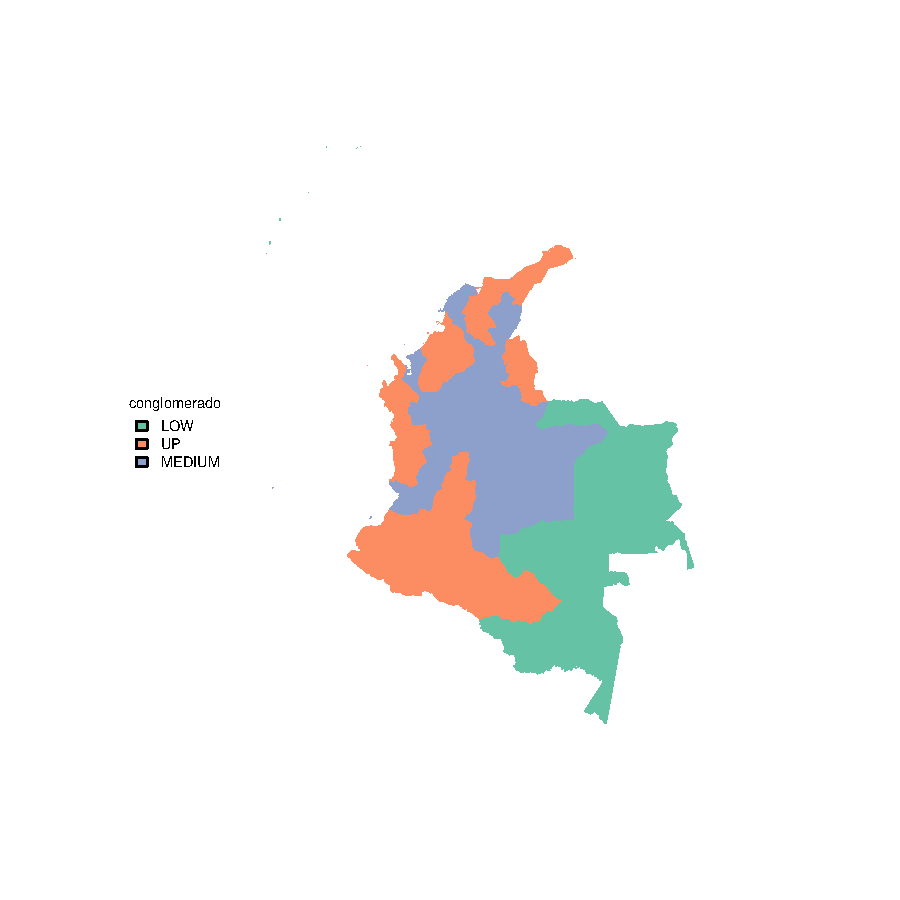
\includegraphics{FinaldeR-plotMap1}

%\end{adjustbox}
\caption{Paises conglomerados segun sus indicadores sociopol\'iticos}\label{clustmap}
\end{figure}

\bibliographystyle{abbrv}
\renewcommand{\refname}{Bibliografia}
\bibliography{Colombia}

\end{document}














\end{document}
